\documentclass[letterpaper,twocolumn,10pt]{article}
\usepackage{usenix2019_v3}

\usepackage{graphicx}
\usepackage{booktabs}
\usepackage{amsmath}

%-------------------------------------------------------------------------------
\begin{document}
%-------------------------------------------------------------------------------

\date{}

\title{\Large \bf Bringing Flexible Data Placement to NVMeVirt:\\
  A Software-Defined FDP SSD for Storage Research}

\author{
{\rm Your Name}\\
Seoul National University
% \and
% {\rm Second Author}\\
% Affiliation
}

\maketitle

%-------------------------------------------------------------------------------
\begin{abstract}
%-------------------------------------------------------------------------------
Flexible Data Placement (FDP) is a recent NVMe feature that lets the host hint
\emph{where} data should be placed on a flash device, so that data with similar
lifetimes can share the same physically reclaimed region and thereby reduce
garbage-collection (GC) write amplification. Studying FDP, however, requires an
FDP-capable device, which are still scarce. We extend NVMeVirt---a
software-defined virtual NVMe device implemented as a Linux kernel
module---with a functional FDP implementation: capability advertisement, the
four FDP log pages and two features, host-directed per-reclaim-unit-handle
(RUH) data placement, and FDP event reporting. The emulated device is driven by
an unmodified Linux NVMe stack and \texttt{nvme-cli}. Using a synthetic
hot/cold workload that models two data lifetimes, we show that FDP placement
reduces write amplification by up to 61\% (a $2.5\times$ improvement in flash
endurance) relative to an identical device with placement disabled, and we
characterize how the benefit depends on over-provisioning and workload skew.
The implementation and evaluation artifacts are publicly available.
\end{abstract}

%-------------------------------------------------------------------------------
\section{Introduction}
%-------------------------------------------------------------------------------
NAND flash cannot overwrite data in place: a page must be erased before it is
rewritten, and erases operate on large blocks. Flash devices therefore write
new data out-of-place and reclaim stale space with a garbage collector (GC)
that must relocate any still-valid pages out of a block before erasing it. This
relocation is pure overhead---it consumes flash program/erase cycles that did
no host work---and is captured by the \emph{write amplification factor} (WAF),
the ratio of bytes written to the media to bytes written by the host. High WAF
degrades throughput, tail latency, and device endurance~\cite{arpachiDusseau18:osbook}.

A long line of work observes that WAF is low when each erase block holds data
of a single \emph{lifetime}: if all the data in a block becomes invalid at
roughly the same time, the block can be reclaimed with little or no
copying~\cite{lifetime:hotcold,multistream:hotstorage14}. The difficulty is
that the device does not know application lifetimes; only the host does.
NVMe \emph{Flexible Data Placement} (FDP)~\cite{fdp:tp4146} closes this gap: the
host attaches a \emph{placement} hint to each write, and the device co-locates
writes that carry the same hint into the same \emph{reclaim unit} (RU). Unlike
Zoned Namespaces (ZNS)~\cite{zns:atc21}, FDP keeps the conventional block
interface---placement is only a hint, and a legacy host still works
unchanged---making it attractive as an incremental path to lifetime-aware
placement.

Studying FDP is hampered by hardware availability. Emulation is the standard
recourse for storage research, and NVMeVirt~\cite{nvmevirt:fast23} is an
attractive base: it presents a real NVMe device to the system at the PCIe layer
from a Linux kernel module, so it is driven by the unmodified kernel NVMe
driver and standard tools. NVMeVirt ships conventional-SSD, ZNS, and key-value
targets, but not FDP.

This paper describes an FDP extension to NVMeVirt and uses it to quantify FDP's
benefit. Our contributions are:
\begin{itemize}
  \item A functional FDP device model for NVMeVirt: capability advertisement in
  Identify, the FDP configuration/usage/statistics/events log pages and the FDP
  and FDP-events features, host-directed placement into per-RUH reclaim units,
  and FDP event reporting (\S\ref{sec:design}).
  \item An evaluation methodology and a synthetic lifetime workload that drive
  the emulated device entirely through the standard NVMe passthrough interface
  (\S\ref{sec:eval}).
  \item A characterization showing up to 61\% WAF reduction from placement, and
  how that benefit varies with over-provisioning and workload skew
  (\S\ref{sec:eval}).
\end{itemize}

%-------------------------------------------------------------------------------
\section{Background}
\label{sec:bg}
%-------------------------------------------------------------------------------

\paragraph{Garbage collection and write amplification.}
A flash translation layer (FTL) maps logical addresses to physical pages and
writes updates to a clean ``write frontier.'' When clean space runs low, GC
selects a victim block, copies its valid pages elsewhere, and erases it. If a
victim holds a mix of soon-to-die and long-lived data, the long-lived pages are
copied repeatedly, inflating WAF. Over-provisioning (OP)---physical capacity in
excess of the exported logical capacity---gives GC slack and lowers WAF, at the
cost of usable space.

\paragraph{NVMe Flexible Data Placement.}
FDP~\cite{fdp:tp4146} adds host-directed placement to the NVM command set. The
host references a \emph{Reclaim Unit Handle} (RUH) through a placement
identifier carried in the write command's directive fields; the device steers
all writes sharing an RUH into the same \emph{Reclaim Unit}, the granularity at
which media is reclaimed. By assigning data of one lifetime class to one RUH,
the host makes each RU fill with similarly-aged data, so reclaiming it copies
little. FDP is exposed through Identify fields, four log pages (configurations,
RUH usage, statistics, events) and two features, and is, crucially, only a
hint: a write without a directive uses a default RUH, so unmodified software
keeps working. This is a key difference from ZNS~\cite{zns:atc21}, which
replaces the block interface with append-only zones, and a generalization of
Streams~\cite{multistream:hotstorage14}.

\paragraph{NVMeVirt.}
NVMeVirt~\cite{nvmevirt:fast23} is a software-defined virtual NVMe device
implemented as a Linux kernel module. It fabricates a virtual PCIe bus and an
NVMe controller backed by a reserved region of host DRAM, and a dispatcher
thread polls the doorbell/BAR registers to process submission queues. Because
the device appears at the PCIe layer, the unmodified in-kernel NVMe driver binds
to it and userspace sees an ordinary \texttt{/dev/nvme*} device. NVMeVirt
includes a page-mapped conventional-SSD FTL (\texttt{conv\_ftl}) with a NAND
timing model and a line-based (super-block) GC; we build our FDP model on it.

%-------------------------------------------------------------------------------
\section{Design and Implementation}
\label{sec:design}
%-------------------------------------------------------------------------------
We add a new build target whose FTL is forked from the conventional-SSD FTL and
extended for FDP. The conventional FTL already provides exactly the machinery
FDP needs---a write frontier per data stream, super-block ``lines'' as the
reclaim granularity, and line-based GC---so the FDP-specific work is to expose
the management interface and to route writes to per-RUH frontiers.

\paragraph{Capability advertisement.}
The controller advertises FDP support in the Identify Controller attributes
(the FDP and Endurance-Group bits), and the namespace advertises the
endurance-group identifier and the preferred-write-granularity fields
(NPWG/NPWA/NOWS) with the I/O-optimization feature bit set so a compliant host
honors them. A single endurance group and a single reclaim group are exposed,
with eight RUHs.

\paragraph{Management interface.}
We implement the four FDP log pages. \emph{Configurations} reports the reclaim
group, RUH count, and reclaim-unit nominal size; \emph{RUH Usage} reports each
RUH's host/controller-specified state; \emph{Statistics} reports host and media
bytes written and bytes erased; and \emph{Events} returns a ring of recent FDP
events. The FDP and FDP-events features are handled in Get/Set Features.
Endurance-group state lives in a single controller-side structure updated on the
dispatcher thread, so no additional locking is required.

\paragraph{Per-RUH placement.}
The write path parses the directive type and specifier from the command. A
write of type \emph{placement} is routed to the write frontier of the addressed
RUH; any other write uses the default RUH. The FTL therefore maintains one open
line per RUH (plus the GC frontier), so writes carrying different placement
identifiers fill different physical lines. An out-of-range placement identifier
is rejected with \emph{Invalid Field in Command}, as required. GC itself is
placement-agnostic: it selects victim lines by valid-page count as before and
relocates survivors to the GC frontier. The benefit therefore comes entirely
from the host \emph{not} mixing lifetimes within a line in the first place.

\paragraph{Statistics and events.}
Host writes increment the host- and media-written counters; GC page copies
increment only the media counter; block erases increment the erase counter.
Thus the Statistics log directly yields $\mathrm{WAF}=\mathrm{MBMW}/\mathrm{HBMW}$.
The device emits an \emph{invalid placement identifier} event on a rejected
placement write and an \emph{implicitly modified reclaim unit} event when GC
reclaims a line the host had written through an RUH, both gated by the
host-settable event mask.

%-------------------------------------------------------------------------------
\section{Evaluation}
\label{sec:eval}
%-------------------------------------------------------------------------------

\subsection{Methodology}
We run NVMeVirt with the FDP target inside a lightweight virtual machine that
boots the host kernel, so the build is exercised by the real Linux NVMe stack
and \texttt{nvme-cli}. The emulated device is 64\,MiB with eight RUHs and
$\approx$7\% intrinsic over-provisioning; writes are 32\,KiB and issued through
the NVMe passthrough interface.

Our primary metric is WAF, read from the FDP Statistics log. WAF depends only on
FTL logic and the workload, not on wall-clock timing, so it is unaffected by
running under emulation; it also maps directly to endurance
($\text{endurance multiplier}=\mathrm{WAF}_{\text{base}}/\mathrm{WAF}_{\text{FDP}}$).

The workload models two lifetime classes with a two-phase generator. First a
\emph{random-order fill} writes the working set once; random order is essential
so that, \emph{without} placement, hot and cold logical addresses are
interleaved into the same physical lines. Then a \emph{churn} phase rewrites the
hot set repeatedly (by default 90\% of writes target the hottest 20\% of the
working set). We compare two configurations on the same device and workload: a
\textbf{baseline} that issues no placement directive (all data to the default
RUH), and \textbf{FDP} that places hot data in one RUH and cold data in another.
WAF is measured as a delta over the churn phase only, so the (WAF$\approx$1) fill
does not dilute the steady-state number. Each measurement uses a fresh device.

\subsection{Write-amplification reduction}
At the operating point (90\% working set, 90\% of writes into the 20\% hot
region), the two configurations issue identical host write volumes but the
baseline writes $6.0\times$ that to the media versus $3.2\times$ for FDP
(Table~\ref{tab:headline})---a 47\% reduction. The baseline pays this cost
because GC repeatedly copies cold pages stranded in hot-dominated lines, exactly
the mixing FDP avoids.

\begin{table}[t]
  \centering
  \caption{Operating point: identical host writes, 47\% less media traffic
  under FDP.}
  \label{tab:headline}
  \begin{tabular}{lrrr}
    \toprule
    & $\Delta$HBMW & $\Delta$MBMW & WAF \\
    \midrule
    Baseline & 20\,MiB & 120\,MiB & 6.02 \\
    FDP      & 20\,MiB & 63\,MiB  & 3.17 \\
    \bottomrule
  \end{tabular}
\end{table}

\subsection{Effect of over-provisioning}
Figure~\ref{fig:op} sweeps the working-set size (and hence free space/OP) at
fixed skew. The FDP benefit is largest at moderate OP: with abundant free space
(75\% working set) GC seldom runs and neither configuration amplifies, while
under extreme pressure (96\%) the device is nearly full and even FDP must copy
to make room. In between, FDP roughly halves WAF (e.g.\ $10.1\times \to 4.6\times$
at 92\% working set). This non-monotonic shape matches the intuition that
placement helps only when GC is both active and avoidable.

\begin{figure}[t]
  \centering
  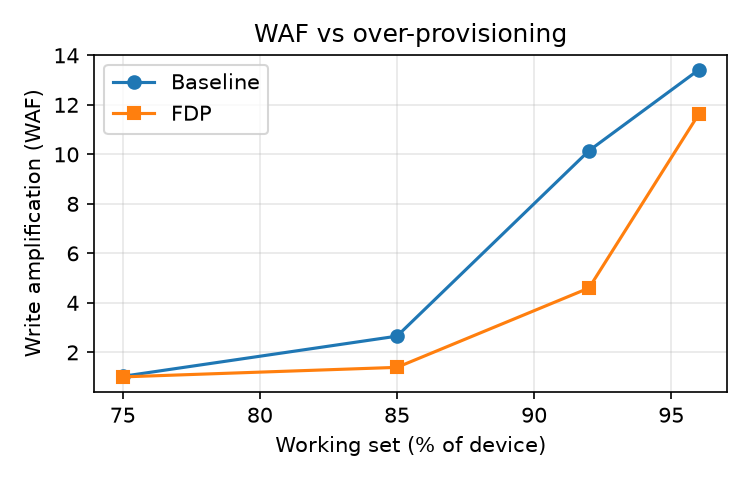
\includegraphics[width=\columnwidth]{op_waf.png}
  \caption{WAF vs.\ over-provisioning (working-set size). FDP's advantage is
  largest at moderate OP and shrinks at both extremes.}
  \label{fig:op}
\end{figure}

\subsection{Effect of workload skew}
Figure~\ref{fig:skew} varies the fraction of writes hitting the hot region at
fixed working set. The baseline WAF is essentially flat ($\approx$5.5)---mixing
lifetimes hurts it regardless of skew---while FDP's WAF falls steadily as the
workload becomes more separable, from $3.95\times$ at 70\% to $2.17\times$ at
95\%. The reduction therefore grows from 31\% to 61\% (up to a $2.5\times$
endurance improvement): the cleaner the lifetime separation the host can
express, the more FDP delivers. Repeated runs at the operating point vary by
about $\pm2\%$, so the trends are well above noise.

\begin{figure}[t]
  \centering
  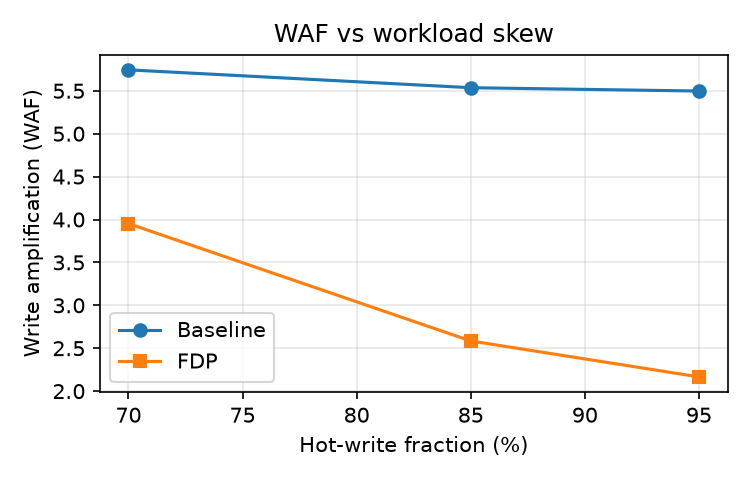
\includegraphics[width=\columnwidth]{skew_waf.png}
  \caption{WAF vs.\ workload skew (hot-write fraction). Baseline is flat; FDP
  improves as lifetimes become more separable.}
  \label{fig:skew}
\end{figure}

\subsection{Discussion and limitations}
The results isolate the placement effect: baseline and FDP differ only in
whether writes carry a directive, on the same device and FTL. Two limitations
follow from our setup. First, we report WAF and endurance, not throughput or
latency: NVMeVirt's timing model is not faithful under pure CPU emulation, so
performance numbers require a bare-metal run. Second, the workload is synthetic;
a two-class hot/cold model is the standard lifetime abstraction, but real
applications (e.g.\ LSM-tree compaction) would strengthen external validity. The
device is intentionally small to make GC reach steady state at a tractable write
volume; the trends are geometry-independent, though absolute WAF scales with OP
and working set.

%-------------------------------------------------------------------------------
\section{Related Work}
%-------------------------------------------------------------------------------
Clustering data by update frequency to lower cleaning cost dates back decades
~\cite{lifetime:hotcold}. Multi-streamed SSDs~\cite{multistream:hotstorage14}
first exposed a host placement hint at the device interface; FDP~\cite{fdp:tp4146}
generalizes streams into a standardized, endurance-group-scoped mechanism. ZNS
~\cite{zns:atc21} attacks the same problem more aggressively by replacing the
block interface with append-only zones, trading host complexity for control;
FDP instead preserves the block interface and treats placement as advisory.
For methodology, FEMU~\cite{femu:fast18} is a QEMU-based NVMe flash emulator,
while NVMeVirt~\cite{nvmevirt:fast23} emulates at the PCIe layer inside the
kernel; we extend the latter because it is driven by the unmodified NVMe stack.

%-------------------------------------------------------------------------------
\section{Conclusion}
%-------------------------------------------------------------------------------
We added a functional NVMe FDP device model to NVMeVirt and used it to quantify
the value of host-directed, lifetime-aware data placement. On a skewed hot/cold
workload, FDP cuts write amplification by up to 61\% ($2.5\times$ endurance)
purely by keeping lifetimes out of each other's reclaim units, and the benefit
depends predictably on over-provisioning and workload skew. The emulator makes
FDP experimentation possible without FDP hardware and on an unmodified host
stack.

%-------------------------------------------------------------------------------
\section*{Availability}
%-------------------------------------------------------------------------------
The FDP extension, the evaluation harness, and the raw data and figures used in
this paper are available in the project repository, a fork of NVMeVirt.

%-------------------------------------------------------------------------------
\bibliographystyle{plain}
\bibliography{paper}

\end{document}
